\documentclass[runningheads]{llncs}
\usepackage[utf8]{inputenc}
\usepackage[T1]{fontenc}
\usepackage{amsmath, amsfonts}
\usepackage{cite, url}
\usepackage{blindtext, todonotes}

\usepackage[english]{babel}
\usepackage{graphicx}
\usepackage{hyperref}


\urldef{\mail}\path|dhuseljic@uni-kassel.de|


\title{Inference in Bayesian Neural Networks}

\begin{document}


\author{Denis Huseljic} 
\institute{Intelligent Embedded Systems, University of Kassel, Germany\\ \mail}

\maketitle
\begin{abstract}
\blindtext
\end{abstract}

% \keywords{Bayesian Neural Networks \and Deep Learning \and Bayesian Inference \and Uncertainty Estimation \and Big Data  }

\section{Introduction}
Due to the improvement in computational performance and the collection of huge amounts of data over the last decade, machine learning (ML) is an important topic in today's society.
It enables the recognition of causalities and patterns in data~\cite{bishop:2006:PRML}.
Due to complex algorithms, autonomous driving and facial recognition are feasible applications and big companies successfully use them from day to day basis~\cite{krizhevsky2012imagenet}.
Furthermore, the use of ML in industry is often unavoidable since the competition in such areas is rapidly evolving.

Deep neural networks (NN) are popular machine learning models which are able to learn complex patterns by means of training examples.
In combination which huge data sets, they achieve superior results in various fields such as image recognition~\cite{efficient_net,multigrain} and natural language processing~\cite{nlp1,nlp2}.
However, although deep NNs are state-of-the-art in many fields of machine learning, they lack in the estimation of uncertainty~\cite{Gal2015Bayesian,Kendall2017Uncertainy}.
They usually make overconfident predictions in situations that they were never trained on.
In practice, this can lead to a lot of problems since uncertainty estimation is an important part of machine learning, and in particular autonomous learning~\cite{Gal2016Active}.
For example, a self driving car should know what it does not know during deployment in practice.
That is, if an image of a sensor is full of noise due to reflections on surfaces in the real world, the deep learning model should return some type of uncertainty which forces the driver to take action~\cite{car_accident}.

In contrast, the Bayesian approach to neural networks~\cite{mackay1992practical,Neal:1995:BLN:922680} and in general Bayesian models offer more detailed information.
In contrast to typical NNs, they incorporate prior knowledge and introduce distributions over they parameters.
As a consequence, they are able to capture uncertainty on instances they were never trained one.
Furthermore, they are also capable to learn from small data sets without the risk of over-fitting.

\todo{Contribution neu, Was ist neu, forschun zusammenfassen}
The main contribution of this work is as follows:
\begin{itemize}
    \item We explain the foundations of neural networks and Bayesian inference.
    Subsequently, we make connections to Bayesian neural networks and discuss their advantages.
    \item We summarize important inference techniques that are used to train such networks. 
    Therefore, we analyze variational inference, expectation propagation and Markov Chain Monte-Carlo methods from the perspective of Bayesian neural networks.
\end{itemize}
Since they offer improved uncertainty estimates, Bayesian neural networks can be used to provide improvement in active learning~\cite{Gal2016Active,hernandez2015probabilistic}, reinforcement learning~\cite{BlundellBBB,Gal2016Dropout}, and various other fields of machine learning.

The rest of this literature review is structured as follows: 
In Section~\ref{sec:foundation}, we introduce foundations that are essential for understanding Bayesian neural networks and their training procedures.
Afterwards in Section~\ref{sec:inference_in_bnn}, we introduce the most important concepts for performing inference and explain state-of-the-art approaches.
Finally in Section~\ref{sec:conclusion_outlook}, we summarize the presented approaches and give an outlook for future work.

\section{Foundations}
\label{sec:foundation}
In the following section, we will provide the necessary introduction to neural networks, Bayesian inference and Bayesian neural networks.
The understanding of these concepts is essential for upcoming methods such as variational inference (Sec.~\ref{sec:variational_inference}), expectation propagation (Sec.~\ref{sec:expectation_propagation}) and Markov chain Monte-Carlo~(Sec.~\ref{sec:mcmc}).

\subsection{Neural Networks}
\label{sec:neural_networks}
Linear classification and regression models are typically based on linear combinations of fixed non-linear basis functions~\cite{bishop:2006:PRML}.
These basis functions have to be determined by the users, and thus are often hard to choose. 
Furthermore, they fail on high dimensional data sets due to the curse of dimensionality~\cite{bishop:2006:PRML}.
Neural Networks (NN)~\cite{HaykinNeuralNetworks} learn such basis functions by incorporating them into their optimization process. 
Consequently, a NN avoids the problems that come with linear models by naturally transforming the data into in an appropriate feature space.

A neural network is inspired by the biological brain~\cite{amit1992modeling}. 
That is, it consists of connected neurons and can learn from experience. 
Typically, it has multiple layers and the ability to extract complex patterns.
Figure~\ref{fig:normal_NN} depicts a multi-layer NN where the nodes represent the input, hidden and output units.
Furthermore, the edges represent adjustable parameters which generally reach large quantities in practice~\cite{efficient_net}.
\begin{figure}
    \centering
    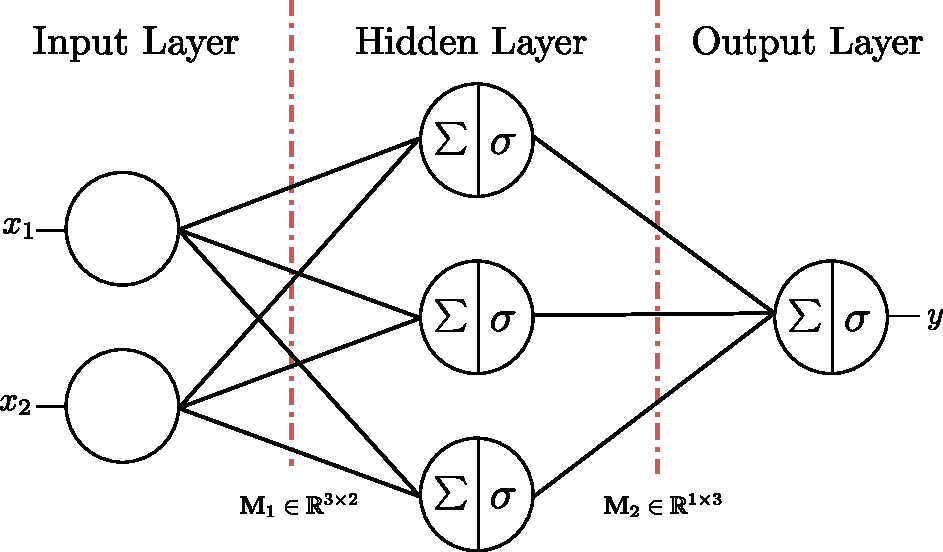
\includegraphics[width=.6\textwidth]{images/NeuralNetwork.pdf}
    \caption{An illustration of a typical neural network with one hidden layer. The nodes represent the neurons and weight matrices are represented by the edges between different layers.
    The summation denotes the matrix multiplication, $\sigma$ denotes an applied activation function and empty nodes define the identity function.
    The weight matrices and their dimensions are denoted below connections between layers.
    }
    \label{fig:normal_NN}
\end{figure}
Such a model is called feed-forward NN because in order to make predictions, it propagates input samples from the first layer (left) to the last layer (right).
We denote the set of all weight matrices between layers of an arbitrary deep NN as $\boldsymbol{\omega} = \{\mathbf{M}_1, \ldots, \mathbf{M}_L\}$.
Thus, for the connections between two layers, we have a $K_l \times K_{l-1}$ dimensional matrix $\mathbf{M}_l$ where $K_l$ depicts the number of neurons in layer $l\in \{0, \ldots, L\}$.
We indicate the input layer with $l=0$ and the output layer with $l = L$.
Furthermore, we have an additional bias vector that we denote with $\mathbf{b}_l$. 

In order to make a prediction for a one hidden layer NN (see Fig.~\ref{fig:normal_NN}), we define the forward propagation as
\begin{align}
    \hat{\mathbf{y}} = \mathbf{M}_2\sigma\left(\mathbf{M}_1 \mathbf{x} + \mathbf{b}_1\right) + \mathbf{b}_2\label{eq:deterministic_forward_prop}
\end{align}
where $\sigma(\cdot)$ is an non-linear activation function (i.\,e., the sigmoid function).
We can generalize Eq.~\ref{eq:deterministic_forward_prop} to more layers by recursively applying matrix multiplications between the output of one layer and the weight matrix leading to the next.
Furthermore, we use a special activation function on the output $\hat{\mathbf{y}}$ which depends on the application (regression or classification). 
Optimization is done with gradient descent and by using the backpropagation algorithm~\cite{Rumelhart:1986we} which allows fast computation of gradients with respect to the weights.
More precise, we compute the errors at the output units of a NN and propagate them back.
In this way, we can achieve an efficient gradient computation in arbitrarily deep networks.

The term deep learning is often used to characterize NNs with a lot of layers. 
In contrast to conventional methods that are limited in working with raw data (i.\,e., image data), deep learning models achieve superior results in various fields like object detection and often do not require methods for feature reduction and extraction.
For example, convolutional neural networks~\cite{krizhevsky2012imagenet} use trainable filters that move over an image in order to extract important features such as edges.
They are based on the concept of the visual cortex and are even able to outperform humans in tasks such as image recognition~\cite{krizhevsky2012imagenet,efficient_net}.

\subsection{Bayesian Inference}
\label{sec:bayesian_inference}
Now we investigate the problem to determine model parameters in a Bayesian way which differs from the usual frequentist perspective.
In a general machine learning setting, we have training samples $\mathbf{X} = \{\mathbf{x}_1, \dots,  \mathbf{x}_N\}$ with their corresponding targets $\mathbf{Y} = \{\mathbf{y}_1, \dots  \mathbf{y}_N\}$. 
Our goal is to determine the parameters $\boldsymbol{\omega}$ of a function such that it captures patterns provided by the data.
In a Bayesian approach, we introduce a prior probability distribution $p(\boldsymbol{\omega})$ which captures our prior belief in the parameters.
For example, we consider a coin flip where we have the parameter set $\boldsymbol{\omega} = \{\mu\}$ and $\mu$ represents the parameter of a Bernoulli distribution (the probability of landing heads).
We do not know the real value of that parameter and in this particular problem, our prior belief might be that we have a fair coin. 
Thus, we introduce a prior $p(\boldsymbol{\omega})$ which takes the form of a $\mathrm{Beta}$ distribution and has its mode at $0.5$.
By observing data, we update that belief by using a likelihood distribution $p\left(\mathbf{Y} | \mathbf{X}, \boldsymbol{\omega} \right)$ which depends on the training data $\left(\mathbf{X}, \mathbf{Y}\right)$. 
If we have a large data set, the likelihood has a big impact on the resulting update and vice versa.
It describes the probability of observing the labels $\mathbf{Y}$ for the given samples $\mathbf{X}$ and some weight $\boldsymbol{\omega}$. 
The corresponding functional form of our likelihood is typically a factorized Gaussian distribution for regression or a factorized Multinoulli distributions for classification.

By combining the likelihood and prior distribution, we obtain the posterior distribution over the parameters given the data according to 
\begin{align}
    p\left(\boldsymbol{\omega} | \mathbf{X}, \mathbf{Y} \right) = \frac{p(\mathbf{Y} | \mathbf{X}, \boldsymbol{\omega})p\left(\boldsymbol{\omega}\right)}{p\left(\mathbf{Y} | \mathbf{X}\right)}.\label{eq:posterior}
\end{align}
The posterior distribution over $\boldsymbol{\omega}$ depicts the most probable parameters given our data.


The denominator $p\left(\mathbf{Y}|\mathbf{X}\right)$ is known as the model evidence or marginal likelihood and is obtained by marginalizing the likelihood and prior with respect to the model parameters $\boldsymbol{\omega}$:
\begin{align}
    p(\mathbf{Y} | \mathbf{X}) = \int p(\mathbf{Y} | \mathbf{X}, \boldsymbol{\omega})p\left(\boldsymbol{\omega}\right) \text{d}\boldsymbol{\omega}\label{eq:model_evidence}.
\end{align}
It ensures that the posterior in Eq.~\ref{eq:posterior} is a valid probability and its sum is equal to one.

In order to make predictions for a new sample $\mathbf{x}^*$ we compute
\begin{align}
    p(\mathbf{y}^*|\mathbf{x}^*, \mathbf{X}, \mathbf{Y}) = \int p\left(\mathbf{y}^* | \mathbf{x}^*, \boldsymbol{\omega} \right) p\left(\boldsymbol{\omega} | \mathbf{X}, \mathbf{Y} \right) \text{d}\boldsymbol{\omega}\label{eq:predictive_distribution}
\end{align}
which is called predictive distribution and yields a distribution over the output $\mathbf{y}^*$.
Note that the first term in Eq.~\ref{eq:predictive_distribution} is not equal to the likelihood we use in the posterior in Eq.~\ref{eq:posterior}.
It depicts the probability distribution of the label $\mathbf{y}^*$ given its new input and some parameters $\boldsymbol{\omega}$, whereas the likelihood considers the whole data set.
Intuitively, we weight predictions higher where the model parameters have a high posterior probability.

Evaluating Eq.~\ref{eq:predictive_distribution} is called \textit{inference} and is the main goal in a Bayesian approach. 
In the coin flip example above, we purposely picked the $\mathrm{Beta}$ distribution for the prior because it is the conjugate of the Bernoulli distribution.
This means that the resulting posterior will also be a $\mathrm{Beta}$ distribution and can be computed analytically.
In contrast, more complex models such as Bayesian neural networks have the problem that the integrals in Eq.~\ref{eq:model_evidence} and Eq.~\ref{eq:predictive_distribution} are intractable.
Thus, we need approximations for the posterior distribution and the predictive distribution.

% Calculating the integrals in Eq.~\ref{eq:model_evidence} and Eq.~\ref{eq:predictive_distribution} can be done analytically for simple models~\cite{bishop:2006:PRML} such as likelihoods with conjugate priors (coin flip example from above).
% However, if the models become more complicated, then these integrals are intractable and hard to approximate.
% Thus, when using deep probabilistic models such as Bayesian Neural Networks, we typically need solid approximations for the posterior \ref{eq:posterior} and the predictive distribution \ref{eq:predictive_distribution}.

\subsection{Bayesian Neural Networks}
\label{sec:bayesian_neural_networks}
A Bayesian Neural Network~\cite{mackay1992practical,Neal:1995:BLN:922680} is similar to an ordinary neural network but avoids the use of point estimates as parameters. 
Instead, it follows an Bayesian approach and defines prior distributions over its weights. 
In particular, we have a set of weights\footnote{Note: We use another the notation for the weights of a Bayesian neural network because now they are random variables.} $\boldsymbol{\omega} = \{\mathbf{W}_1,\ldots, \mathbf{W}_L\}$ and introduce the prior distributions $p(\mathbf{W}_l)$ for each layer $l$. 
For simplicity, we assume point estimates for the bias terms $\mathbf{b}_l$. 
\begin{figure}
    \centering
    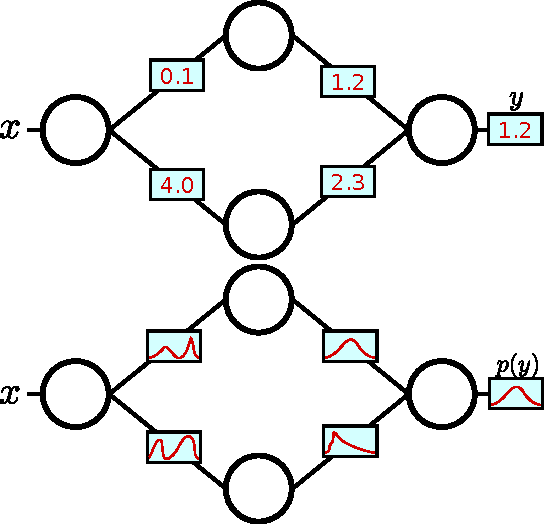
\includegraphics[width=.55\textwidth]{images/BayesianNeuralNetwork.pdf}
    \caption{Illustration of a deterministic neural network (left) and Bayesian neural network (right). The weights of the ordinary NN are defined by point estimates which as well results in a point estimate for the prediction $y$. In contrast, the Bayesian NN defines a distribution over its weights and thus we obtain a distribution $p(y)$ for the output.}
    \label{fig:bayesian_neural_network}
\end{figure}

The main goal in such a settings is to compute the posterior distribution $p\left(\boldsymbol{\omega} | \mathbf{X}, \mathbf{Y} \right)$ which is defined by Eq.~\ref{eq:posterior}.
Furthermore by using Eq.~\ref{eq:predictive_distribution}, we would obtain a predictive distribution for new inputs $\mathbf{x}^*$.
This is illustrated in Fig.~\ref{fig:bayesian_neural_network}.

In practice, we obtain the predictive distribution~\ref{eq:predictive_distribution} by Monte-Carlo integration.
That is, we make multiple forward propagations with weights that are sampled independently from the posterior (its current approximation) which leads to a output distribution. An example for this is shown in Fig.~\ref{fig:uncertainty_example}.

By adding distributions over the weights, our NN is able to capture epistemic uncertainty.
The term \textit{epistemic uncertainty} (knowledge uncertainty) depicts the uncertainty in the model parameters and can be reduced by observing more data. 
The counterpart \textit{aleatoric uncertainty} (dice players uncertainty) characterizes the uncertainty that can not be reduced (e.\,g., sensor noise). 
\begin{figure}
    \centering
    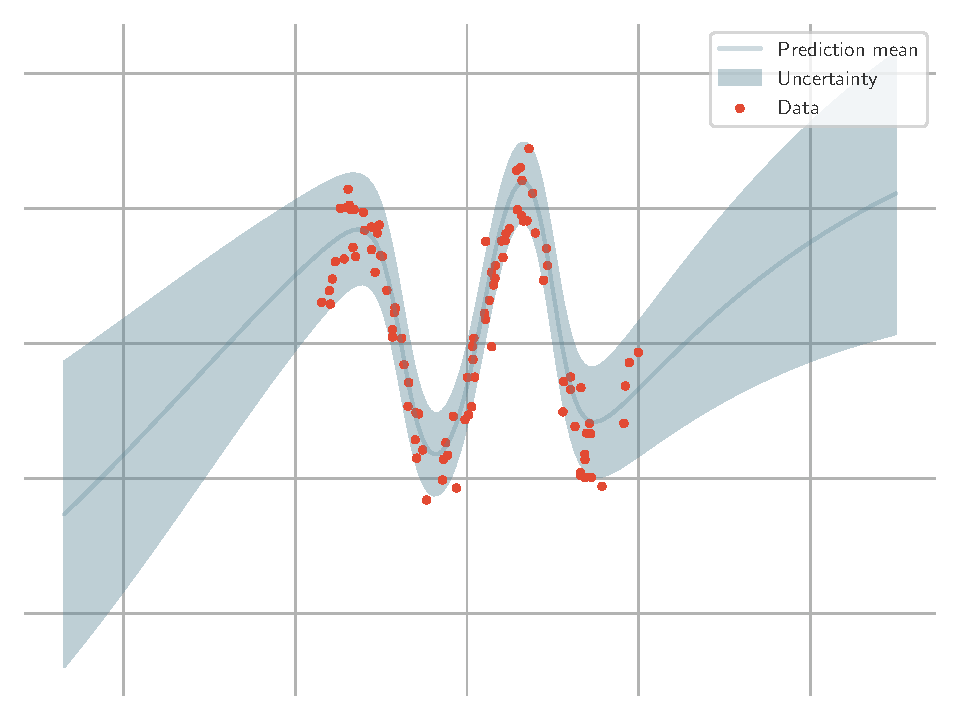
\includegraphics[width=.7\textwidth]{images/uncertainty_example.pdf}
    \caption{The predictive distribution inferred by a Bayesian Neural Network for a simple regression task. As a result, we see increasing uncertainty in areas where no data was observed (epistemic) as well as uncertainty that is due to noisy measurements (aleatoric). The BNN was trained on a toy data set with Bayes-by-Backprop, a method that we explain in Sec.~\ref{sec:bayes_by_backprop}.
    In order to make these predictions, we made $100$ forward propagations, each yielding a different result, and computed their mean and standard deviation. Therefore, we had to sample $100$ weights from the approximation of the posterior distribution $p(\boldsymbol{\omega}| \mathbf{X}, \mathbf{Y})$.}
    \label{fig:uncertainty_example}
\end{figure}

We obtain a lot of useful properties by adding priors over the weights.
However unlike the prior distribution we used in our coin flip example, the priors in a BNN are hard to interpret and it is difficult to incorporate prior knowledge.~\cite{Neal:1995:BLN:922680}.
Furthermore, the complexity of BNNs inhibit the analytic computation of the required posterior given by Eq.~\ref{eq:posterior} due to the integration with respect to the large number of parameters in the denominator.
Thus, we have to use approximations and we will introduce several approaches in the next section.

\section{Inference in Bayesian Neural Networks}
\label{sec:inference_in_bnn}
In order to train a Bayesian neural network, the main goal is to determine the posterior distribution given by
\begin{align*}
    p\left(\boldsymbol{\omega} | \mathbf{X}, \mathbf{Y} \right) = \frac{p(\mathbf{Y} | \mathbf{X}, \boldsymbol{\omega})p\left(\boldsymbol{\omega}\right)}{\underbrace{p\left(\mathbf{Y} | \mathbf{X}\right)}_{\text{intractable}}},
\end{align*}
where the model evidence $p(\mathbf{Y}|\mathbf{X})$ from  Eq.~\ref{eq:model_evidence} is intractable due to the integral with respect to the parameters $\boldsymbol{\omega} = \{\mathbf{W}_1, \ldots,\mathbf{W}_L\}$.
Therefore, we make use of approximate inference techniques~\cite{Gal2016Uncertainty} which are typically employed when working with intractable distributions. 

The functional form of the likelihood $p(\mathbf{Y} | \mathbf{X}, \boldsymbol{\omega})$ and prior $p\left(\boldsymbol{\omega}\right)$ has to be chosen by the user.
For example, the likelihood can be given as
\begin{align}
    p(\mathbf{Y} | \mathbf{X}, \boldsymbol{\omega}) = \prod_{i=1}^N p\left(\mathbf{y}_i | f^{\boldsymbol{\omega}}(\mathbf{x}_i) \right),
\end{align}
where $f^{\boldsymbol{\omega}}(\mathbf{x}_i)$ denotes the output of the network and $p\left(\mathbf{y}_i|f^{\boldsymbol{\omega}}(\mathbf{x}_i)\right)$ is a task specific distribution.
That is, in regression tasks we often assume a Gaussian distribution $p\left(\mathbf{y}_i|f^{\boldsymbol{\omega}}(\mathbf{x}_i)\right) = \mathcal{N}\left(\mathbf{y}_i | f^{\boldsymbol{\omega}}(\mathbf{x}_i) , \sigma^2 \right)$ where $\sigma^2$ is a hyperparameter.
In classification tasks, $f^{\boldsymbol{\omega}}(\mathbf{x}_i)$ returns a vector of probabilities (we use a softmax function in the last layer), and thus we apply it to a Multinoulli distribution $p\left(\mathbf{y}_i|f^{\boldsymbol{\omega}}(\mathbf{x}_i)\right) = \operatorname{Multinoulli}(\mathbf{y}_i |f^{\boldsymbol{\omega}}(\mathbf{x}_i))$.
Moreover, the prior distribution can be formulated in a factorized way given by
\begin{align}
    p\left(\boldsymbol{\omega}\right)=\prod_{l = 1}^{L}\prod_{i=1}^{K_{l}}\prod_{j=1}^{K_{l-1}} \mathcal{N} \left(w_{ij, l} \mid \mu, \sigma^2\right), \label{eq:prior_factorized}
\end{align}
where $w_{ij,l}$ represents the weight of neuron $j$ in layer $l-1$ to neuron $i$ in layer $l$. The parameters $\mu$ and $\sigma^2$ have to be provided by the user and are typically set to $0$ and $1$.
Additionally, one can adapt theses parameters in order to force different behaviors. 

% page 462 in bishop
In general, there are two main approaches for the approximation of the posterior $p\left(\boldsymbol{\omega} | \mathbf{X}, \mathbf{Y} \right)$, namely deterministic and stochastic methods~\cite{bishop:2006:PRML}.
\textit{Deterministic methods} estimate the intractable posterior by assuming a more simple tractable distribution.
Based on that, these often optimize dissimilarity measures and therefore the inference problem is transformed into an optimization problem.
Such methods scale well with large applications and can be implemented efficiently.
However, since they assume simpler tractable distributions, they are never able to generate (sample) exact results from our posterior.
In contrast, \textit{stochastic methods} are able to generate exact results if unlimited computational power is given.
Despite that, they are only suitable in application with few parameters because time and computational resources are often limited.
Therefore, we will mainly focus on deterministic methods.\footnote{Different implementations of the algorithms that are mentioned below can be found at \url{https://git.ies.uni-kassel.de/dhuseljic/bayesian-neural-networks}.}

\subsection{Variational Inference}
\label{sec:variational_inference}
One popular approach for approximate inference is \textit{variational inference} (VI)~\cite{blei2017variational} which belongs to the deterministic methods.
Instead of computing the posterior analytically, we define a \textit{variational distribution} $q_\theta(\boldsymbol{\omega})$ that has a simple form and is defined by the parameters $\theta$.
As a result, we are able to sample the set of weights $\boldsymbol{\omega}$ from the variational $q_\theta(\boldsymbol{\omega})$ and avoid the problems that come with the posterior.
Subsequently, we transform our inference problem into an optimization problem by minimizing the Kullback-Leibler (KL) divergence~\cite{Kullback51klDivergence} with respect to the parameters $\theta$ given by
\begin{align}
    \text{KL}\left( q_\theta(\boldsymbol{\omega}) \| p(\boldsymbol{\omega} | \mathbf{X}, \mathbf{Y})\right) &= - \int q_{\theta}(\boldsymbol{\omega}) \ln \left(\frac{p(\boldsymbol{\omega} | \mathbf{X}, \mathbf{Y})}{q_{\theta}(\boldsymbol{\omega})}\right) \text{d}\boldsymbol{\omega}.\label{eq:kl_divergence}
    %. \\ &= \mathbb{E}_{q_\theta(\boldsymbol{\omega})}\left[\ln q_{\theta}(\boldsymbol{\omega})\right] - \mathbb{E}_{q_\theta(\boldsymbol{\omega})}\left[\ln p(\boldsymbol{\omega} | \mathbf{X}, \mathbf{Y})\right]
\end{align}
Intuitively, it can be seen as a dissimilarity measure between two distributions and is a non-negative quantity. Thus, minimizing the KL-divergence w.r.t $\theta$ induces similarity between the variational distribution $q_\theta(\boldsymbol{\omega})$ and the posterior distribution $p(\boldsymbol{\omega} | \mathbf{X}, \mathbf{Y})$.

By reformulating Eq.~\ref{eq:kl_divergence} (see Appendix), we are able to obtain an equivalent optimization problem where we have to minimize the negative evidence lower bound (ELBO) given by
\begin{align}
    \mathcal{F}(\theta) &= - \int q_\theta(\boldsymbol{\omega}) \ln p \left(\mathbf{Y} | \mathbf{X}, \boldsymbol{\omega}\right) \text{d}\boldsymbol{\omega} +
    \text{KL}\left(q_\theta(\boldsymbol{\omega}) || p(\boldsymbol{\omega}) \right). \label{eq:elbo} 
    \\
    &= - \mathbb{E}_{q_\theta(\boldsymbol{\omega})}\left[ \ln p \left(\mathbf{Y} | \mathbf{X}, \boldsymbol{\omega}\right)\right] +
    \text{KL}\left(q_\theta(\boldsymbol{\omega}) || p(\boldsymbol{\omega}) \right). \label{eq:elbo_loss_expectation}
\end{align}
In Eq.~\ref{eq:elbo_loss_expectation} we see that the ELBO is a combination of the negative expected log likelihood and the KL-Divergence of our variational and prior distribution.
The first term forces the weights to explain the observed data whereas the second term forces the variational distribution to be close to the prior. 
That is, the KL-divergence can be understood as a regularization term which penalizes high distances from the variational $q_\theta(\boldsymbol{\omega})$ to the prior $p(\boldsymbol{\omega})$.
For example, if the prior distribution given by Eq.~\ref{eq:prior_factorized} uses a small variance, than the KL-divergence has a large contribution to the overall error in Eq.~\ref{eq:elbo_loss_expectation} which leads to a strong regularization. 
Thus, the variance in the prior can be seen as a hyperparameter for regularization.

The specific functional form of the variational distribution $q_\theta$ is an important user specific choice.
It has to be a simple distribution such that we can efficiently sample from it.
Additionally, it needs to be expressive in the sense that it is able to provide a good approximation to the true posterior.
One popular approach is to use a factorized distribution~\cite{BlundellBBB,Graves2011Practical,hernandez2015probabilistic} which is obtained by introducing a simple distribution (i.\,e., Gaussian) for every weight and taking their product.
Similarly to the likelihood, it uses an independence assumption between the weights which is often called mean field assumption~\cite{blei2017variational}.
Thus, a BNN might take a variational distribution as 
\begin{align}
    q_\theta\left(\boldsymbol{\omega}\right) = \prod_{l=1}^{L}\prod_{i=1}^{K_l}\prod_{j=1}^{K_{l-1}} \mathcal{N}\left( w_{ij,l} \mid \theta^\mathrm{mean}_{ij,l}, \theta^\mathrm{var}_{ij,l}\right)\label{eq:variational_factorized}
\end{align}
where $\theta^\mathrm{mean}_{ij,l}$ and $\theta^\mathrm{var}_{ij,l}$ are elements of the variational parameters $\theta$ for the mean and variance of a connection in the NN. 
We can sample from that distribution in an easy way~\cite{bishop:2006:PRML} with the drawback that we loose weight correlations which is due to the independence assumption. This is illustrated in Figure~\ref{fig:correlation_loss}.
\begin{figure}
    \centering
    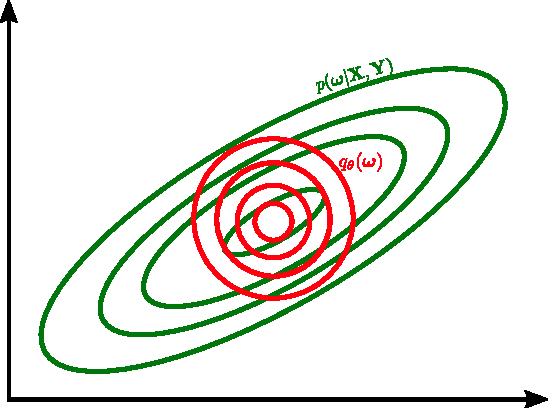
\includegraphics[width=.6\textwidth]{images/loosing_correlations.pdf}
    \caption{An example on the independence drawback. The factorized variational distribution $q_\theta(\boldsymbol{\omega})$ (red) can not capture the correlations provided by the posterior distribution $p(\boldsymbol{\omega} | \mathbf{X}, \mathbf{Y})$ (green).}
    \label{fig:correlation_loss}
\end{figure}

In this way, we obtain a loss function for our neural network which we need to optimize with respect to the variational parameters $\theta$ (i.\,e. every $\theta^\mathrm{mean}_{ij,l}$ and $\theta^\mathrm{var}_{ij,l}$). 
Therefore, we only compute derivatives instead of the integral in the model evidence (Eq.~\ref{eq:model_evidence}) which is usually easier due to existing algorithms like backpropagation. 
However, ordinary VI does not scale to large data sets and yields problems when dealing with high model complexity~\cite{Gal2016Uncertainty}.
In particular, the expected log likelihood term in Eq.~\ref{eq:elbo_loss_expectation} still needs an integration over all model parameters, we need to compute this expectation for each entry $(\mathbf{x}_i, \mathbf{y}_i)$ in our training data and we have to derive its gradient.
In order to tackle these problems, we will introduce several approximation schemes in the following sections.

\subsubsection{Practical Variational Inference}
\label{parctical_vi}
One of the first well working approaches (in a deep learning context) was introduced by Graves~\cite{Graves2011Practical}.
He derives the expected log likelihood and KL-divergence, which yield the ELBO loss given in Eq.~\ref{eq:elbo_loss_expectation}, and its gradients for different choices of variational posteriors $q_\theta(\boldsymbol{\omega})$ and priors $p(\boldsymbol{\omega})$.
All distributions were defined in a factorized way as given by Eq.~\ref{eq:prior_factorized} and Eq.~\ref{eq:variational_factorized}.

In order to compute the intractable expected log likelihood, he uses Monte-Carlo integration defined by
\begin{align}
    \mathbb{E}_{q_\theta(\boldsymbol{\omega})}\left[ \ln p \left(\mathbf{Y} \middle| \mathbf{X}, \boldsymbol{\omega}\right)\right] &\approx \frac{1}{K} \sum_{k=1}^K \ln p\left(\mathbf{Y} \middle| \mathbf{X, \boldsymbol{\omega}}^{(k)}\right)\label{eq:montecarlo_expectation}
    %\\ &= \frac{1}{S} \sum_{i=1}^{N} \sum_{k=1}^{S} \ln p\left(\mathbf{y}_i | f^{{\boldsymbol{\omega}}^{k}} (\mathbf{x}_i) \right)
\end{align}
where $\boldsymbol{\omega}^{(k)}$ are samples drawn independently from $q_\theta(\boldsymbol{\omega})$ and $K$ is the total number of Monte-Carlo samples which needs to be specified by the user.
This leads to stochastic gradients which must be considered in the training procedure (i.\,e., by the optimizer).
Furthermore, he uses sub-sampling techniques in order to avoid computation over large data sets.

For the computation of the KL-Divergence, he uses a closed form that is obtained by assuming the two Gaussian distributions for prior (Eq.~\ref{eq:prior_factorized}) and variational (Eq.~\ref{eq:variational_factorized}) given by
\begin{align}
\mathrm{KL}(q_\theta(\boldsymbol{\omega})\|p(\boldsymbol{\omega})) =
%\sum_{i=1}^{W} \ln \frac{\sigma}{m_i} + \frac{1}{2\sigma^2} \left((\mu - m_i)^2 + v_i^2 - \sigma^2\right)\\
\sum_{l=1}^{L}\sum_{i=1}^{K_l}\sum_{j=1}^{K_{l-1}} \ln \frac{\sigma}{\theta^{\mathrm{mean}}_{ij,l}} + \frac{1}{2\sigma^2} \left(( \theta^{\mathrm{mean}}_{ij,l}-\mu )^2 + \theta^{\mathrm{var}}_{ij,l} - \sigma^2\right)
%\sum_{l=1}^{L}\sum_{i=1}^{K_l}\sum_{j=1}^{K_{l-1}} \ln \frac{\sigma}{m_{ij,l}} + \frac{1}{2\sigma^2} \left((\mu - m_{ij,l})^2 + v_{ij,l}^2 - \sigma^2\right)
% \sum_{l=1}^{L}\sum_{i=1}^{K_l}\sum_{j=1}^{K_{l-1}} \ln \frac{\sigma_{ij,l}}{m_{ij,l}} + \frac{1}{2\sigma_{ij,l}^2} \left((\mu_{ij,l} - m_{ij,l})^2 + v_{ij,l}^2 - \sigma_{ij,l}^2\right)
\end{align}
where the summations iterate over all connections in our BNN and $\mu$ and $\sigma$ are defined as the parameters for a Gaussian prior.
We avoid indices over the prior parameters to keep the notation uncluttered and because we assume the same prior for each weight in our network.
However, by adding indices one could use different prior distributions in different layers.

Graves introduced the first approach that works well with complex models and large data sets.
However, in practical application his VI approach does not perform well due to noisy gradient estimations and missing weight correlations.
The former is due to taking the derivative of the Monte-Carlo integration in Eq.~\ref{eq:montecarlo_expectation} and the latter is due to the factorized assumption for the variational distribution (see Fig.~\ref{fig:correlation_loss}).

\subsubsection{Bayes-by-Backprop}
\label{sec:bayes_by_backprop}
Extending on the work of Graves, Blundell et al.~\cite{BlundellBBB} introduced \textit{Bayes-by-Backprop}.
Likewise, it is also based on the use of derivatives to optimize the ELBO loss.
However, they tackled the problem of high variance from the stochastic gradients. 
Thus, they exploit the \textit{local reparametrization trick} that was proposed by Kingma et al.~\cite{Kingma:2015:VDL:2969442.2969527}, which was never used in the context of Bayesian neural networks~\cite{kingma2013autoencoding}.

The reparametrization trick expresses that under certain assumptions the derivative of an expectation can be reformulated to an expectation of a derivative. 

\begin{theorem}
\label{the:reparam_trick}
\textbf{Reparametrization Trick.} Let $\epsilon$ be a random variable which is distributed according to a parameter free distribution $q(\epsilon)$ and let $\boldsymbol{\omega} = t(\theta, \epsilon)$ where $t(\theta, \epsilon)$ is a deterministic function. Furthermore, we assume that small changes in $q(\epsilon)$ are equal to small changes in $q_\theta(\boldsymbol{\omega})$: $q(\epsilon)\mathrm{d}\epsilon = q_\theta(\boldsymbol{\omega})\mathrm{d}\boldsymbol{\omega}$.
Then the following applies for an arbitrary function $f(\boldsymbol{\omega}, \theta)$:
\begin{align}
\frac{\partial}{\partial\theta} \mathbb{E}_{q_\theta(\boldsymbol{\omega})} \left[f(\boldsymbol{\omega}, \theta)\right]= 
\mathbb{E}_{q(\epsilon)}\left[ \frac{\partial f(\boldsymbol{\omega}, \theta)}{\partial\boldsymbol{\omega}}\frac{\partial\boldsymbol{\omega}}{\partial\theta} + \frac{\partial f(\boldsymbol{\omega}, \theta)}{\partial \theta}\right].\label{eq:reparam_trick}
\end{align}
Proof. See \cite{BlundellBBB}.
\end{theorem}
Using Theorem~\ref{the:reparam_trick}, we transform the derivative of our objective function from Eq.~\ref{eq:elbo_loss_expectation}, to
\begin{align}
    \frac{\partial}{\partial\theta}\mathcal{F}(\theta) &= \frac{\partial}{\partial\theta}\int q_\theta(\boldsymbol{\omega}) \ln \frac{q_\theta(\boldsymbol{\omega})}{p(\boldsymbol{\omega})p(\mathbf{Y} | \mathbf{X}, \boldsymbol{\omega})}\mathrm{d}\boldsymbol{\omega} \\
    &= \frac{\partial}{\partial\theta}\mathbb{E}_{q_\theta(\boldsymbol{\omega})}\left[ \ln \frac{q_\theta(\boldsymbol{\omega})}{p(\boldsymbol{\omega})p(\mathbf{Y} | \mathbf{X}, \boldsymbol{\omega})} \right]\label{eq:applied_reparam} \\
    &\overset{\eqref{eq:reparam_trick}}{=}
    \mathbb{E}_{q(\epsilon)}\left[ \frac{\partial f(\boldsymbol{\omega}, \theta)}{\partial\boldsymbol{\omega}}\frac{\partial\boldsymbol{\omega}}{\partial\theta} + \frac{\partial f(\boldsymbol{\omega}, \theta)}{\partial \theta} \right]
    \label{eq:elbo_bayes_by_backprop}
\end{align}
with $f(\boldsymbol{\omega}, \theta) = \ln q_\theta(\boldsymbol{\omega}) / p(\boldsymbol{\omega})p(\mathbf{Y} | \mathbf{X}, \boldsymbol{\omega})$ and $\boldsymbol{\omega} = t(\theta, \epsilon)$.
That is, we rewrite the expectation that is taken with respect to the variational distribution $q_\theta(\boldsymbol{\omega})$ so that it is independent of all parameters $\theta$.
For example, we might assume $q(\epsilon)$ to be a unit Gaussian and apply the deterministic function $t(\theta, \epsilon) = \mu + \sigma \cdot \epsilon$.
This leads to unbiased Monte-Carlo gradients~\cite{BlundellBBB} which usually have much lower variance since we do not have to compute the derivative of an approximated expectation but approximate a derivative.

Note, until this point we only considered the computation of the derivatives with respect to all parameters.
In order to estimate the true loss, we use Monte-Carlo integration which results in
\begin{align}
    \mathcal{F}(\theta) &=  \mathbb{E}_{q_\theta(\boldsymbol{\omega})}\left[ \ln \frac{q_\theta(\boldsymbol{\omega})}{p(\boldsymbol{\omega})p(\mathbf{Y} | \mathbf{X}, \boldsymbol{\omega})} \right]\label{eq:applied_reparam} \\
    &\approx \frac{1}{K}\sum_{k=1}^K \ln q_\theta(\boldsymbol{\omega}^{(k)}) - \ln p(\boldsymbol{\omega}^{(k)}) - \ln p(\mathbf{Y} | \mathbf{X}, \mathbf{\boldsymbol{\omega}}^{(k)}), 
\end{align}
where $\boldsymbol{\omega}^{(k)}$ are drawn independently from our variational posterior $q_\theta(\boldsymbol{\omega})$ and $K$ is the number of Monte-Carlo samples.
By implementing this loss and using the deterministic function $\boldsymbol{\omega} = t(\theta, \epsilon)$ to obtain samples from our variational distribution, we can easily train a BNN by means of automatic differentiation.

Note, we do not have an explicit KL-divergence term between the variational and prior distribution as in Eq.~\ref{eq:elbo_loss_expectation}.
This allows several combinations of distributions for the prior as well, e.\,g., the variational distribution.
Further, Blundell et al. propose a Gaussian mixture prior for their experiments given by
\begin{align}
    p(\boldsymbol{\omega}) = \prod_{l=1}^{L}\prod_{i=1}^{K_l}\prod_{j=1}^{K_{l-1}} \pi\mathcal{N}(w_{ij,l} | 0, \sigma_1^2) + (1 - \pi)\mathcal{N}(w_{ij,l}| 0, \sigma_2^2)\label{eq:mixture_prior}
\end{align}
where $\pi$ is the probability of one mixture component. 
The variances $\sigma_1^2$ and $\sigma_2^2$ are set so that $\sigma_1^2 \gg \sigma_2^2$ and thus we obtain a Gaussian which has a tight peek centered around zero.
By using Eq.~\ref{eq:mixture_prior}, they empirically showed that they can avoid hyperparameter optimization of the prior distribution.

Shridhar et al.~\cite{shridhar2019comprehensive} proposed an extension to a Bayesian CNN by adding Gaussian distributions over parameters of filters.
They also achieved similar results as deterministic dropout CNN architectures on MNIST~\cite{lecun-mnisthandwrittendigit-2010} and Cifar-10~\cite{cifar}.

\subsubsection{Dropout Variational Inference}
\label{sec:dropout_inference}
The approaches above are usable with complex models due to factorized distributions for prior/posterior and are also able to process large data sets due to sub-sampling approaches.
Furthermore, even though they do not achieve better results than deterministic models, they obtain similar ones with the extension of uncertainty estimates.

However, the complexity of modern deep learning models are often as big as the memory of a GPU allows.
By considering the methods above, we already double that complexity.
For example, if we assume simple Gaussian distributions for both prior and variational, we obtain mean and variance parameters for each connection.
That is a problem when applying Bayesian NNs to state-of-the-art architectures.
Furthermore, until now we were not able to design correlations between weights which generally leads to superior predictive performance~\cite{krizhevsky2012imagenet}.

\todo{Wohin? Ggf. von oben den text mit runter kopieren}Gal et al.~\cite{Gal2016Uncertainty} noticed these problems that occur when using Bayesian models in practice. 
Furthermore, he discovered practical methods in Bayesian neural networks~\cite{Gal2016Dropout} with the help of existing techniques such as dropout~\cite{Srivastava:2014:DSW:2627435.2670313}.
With the help stochastic regularization techniques (SRT), one is able to estimate uncertainty in a NN.
Therefore, we will first introduce dropout which is a commonly used SRT in most deep learning models.

Now, we consider a deterministic neural network with one hidden layer to illustrate the use of dropout.
Its (also deterministic) model parameters are defined by the matrices $\mathbf{M}_1 \in \mathbb{R}^{K_1\times K_0}$, which represent all connections\footnote{Recall: $K_i$ is the number of neurons in layer $i$.} from the input layer $0$ to hidden layer  $1$, and $\mathbf{M}_2 \in \mathbb{R}^{K_2\times K_1}$, which represents all connections form the hidden layer $1$ to the output layer $2$.
Furthermore, we define bias vectors in each layer which we denote with $\mathbf{b}_1 \in \mathbb{R}^{K_1}$ and $\mathbf{b}_2\in \mathbb{R}^{K_2}$.

The output of the first layer is determined by $\mathbf{h} = \sigma \left(\mathbf{M}_1\mathbf{x} + \mathbf{b}_1\right)$ where $\sigma$ depicts some kind of nonlinear function (i.\,e. $\sigma(x) = \tanh(x)$).
Furthermore, the whole network output is defined as $\hat{\mathbf{y}} = \mathbf{M}_2\mathbf{h} + \mathbf{b}_2$ where we generally include an additional activation function based on the type of application (classification or regression).
This results in a complete forward propagation defined by Eq.~\ref{eq:deterministic_forward_prop}.
Typically, the elements of the weight matrices are adapted during training, for example by gradient descent.

Intuitively when applying dropout, we drop units from our network by setting their output values to zero randomly.
Mathematically, this is done by sampling two binary vectors $\boldsymbol{\epsilon}_1$ and $\boldsymbol{\epsilon}_2$ independently from a Bernoulli distribution $\mathrm{Bern}(p)$ where $p$ represents the probability of a neuron being dropped.
Thus, by using dropout, the output of the first layer is defined as $\mathbf{h} = \sigma\left( \mathbf{M_1}\hat{\mathbf{x}} + \mathbf{b}_1\right)$ where $\hat{\mathbf{x}} = \mathbf{x} \odot \boldsymbol{\epsilon}_1$.
Similarly, the output of the second layer is $\hat{\mathbf{y}} = \mathbf{M}_2\hat{\mathbf{h}} + \mathbf{b}_2$ where $\hat{\mathbf{h}} = \mathbf{h} \odot \boldsymbol{\epsilon}$.
The $\odot$-operator defines the hadamard product (element-wise multiplication).
Thereby, we randomly add noise to the units of our network which leads to regularization, and therefore to a better generalization.
At training, we apply dropout for every new input sample and use the corresponding output for the gradient descent algorithm.
At test time, we usually stop the dropout procedure and use the original units scaled by the factor $1 / \left(1 - p)\right)$. 
We will see that using dropout at test time results in several advantages.

Gal et al.~\cite{Gal2016Uncertainty} showed that using stochastic regularization techniques in an ordinary neural network, can be interpreted as an variational Bayesian approximation in an Bayesian NN with equivalent network architectures.
In order to show this, we transform the dropouts noise, that is currently added to samples in the feature space according to 
\begin{align*}
    \hat{\mathbf{y}} = \mathbf{M}_2\hat{\mathbf{h}} 
    = \mathbf{M}_2 \left( \boldsymbol{\epsilon}_2 \odot \mathbf{h}   \right) 
    = \mathbf{M}_2 \left( \mathrm{diag}\left(\boldsymbol{\epsilon}_2\right) \mathbf{h}   \right) 
    = \left(\mathbf{M}_2  \cdot\mathrm{diag}\left(\boldsymbol{\epsilon}_2\right)\right) \mathbf{h}    
\end{align*}
where $\mathrm{diag}(\cdot)$ transforms a vector into a diagonal matrix.
This can be done similarly for the other weight matrix $\mathbf{M}_1$. 
Thereby, dropout is now applied to the parameter space and we can interpret both matrices $\mathbf{W}_1 = \mathbf{M}_1  \cdot\mathrm{diag}\left(\boldsymbol{\epsilon}_1\right)$ and $\mathbf{W}_2 = \mathbf{M}_2  \cdot\mathrm{diag}\left(\boldsymbol{\epsilon}_2\right)$ as stochastic samples from a variational distribution $q(\boldsymbol{\omega})$.
Gal refers the samples $\boldsymbol{\omega} = \{\mathrm{diag}(\boldsymbol{\epsilon}_1)\mathbf{M}_1,\mathrm{diag}( \boldsymbol{\epsilon}_2)\mathbf{M}_2 \}$ to a \textit{Bernoulli variational distribution} or \textit{dropout variational distribution}.
It can be interpreted as a mixture of two Gaussians in which the first component has its mean fixed at zero according to $\mathcal{N}(0, \sigma^2)$. The second component is fixed at its weight value $\mathcal{N}(m,\sigma^2)$, where $m$ is an element of one of the deterministic matrices $\{\mathbf{M}_1, \dots, \mathbf{M}_L\}$.
Both components have a tiny variance $\sigma^2$~\cite{Gal2015Bayesian} and the mixing coefficient is defined by the dropout rate.

In order to show that dropout in an ordinary NN is equivalent to VI in a BNN, we investigate the usual VI objective that is given by Eq.~\ref{eq:elbo_loss_expectation}.
Note, the objective function of a dropout neural network (e.\,g., mean squared error) with weight decay has a similar form.
In particular, we set the value of our regularization term equal to the value of the KL-divergence as
\begin{align}
\mathrm{KL}\left(q_\theta(\boldsymbol{\omega}))\|p(\boldsymbol{\omega})\right) = \lambda_1 \|\mathbf{M}_1\|^2+ \lambda_2 \|\mathbf{M}_2\|^2 + \lambda_3 \|\mathbf{M}_3\|^2
\end{align}
where $\lambda_1, \lambda_2, \lambda_3 \in \mathbb{R}$ are regularization factors.
Gal showed~\cite{Gal2016Uncertainty} that in order to obtain an equivalent VI objective, we need to set the regularization factors to 
\begin{align}
    \lambda_i = \frac{l_i^2 (1 - p_i)}{2 N \tau},
\end{align}
where $l_i$ is called lengthscale, $\tau$ is the precision of the prior distributions and $p_i$ is the probability for a neuron to be dropped in layer $i$. 
Low values for the lengthscale allow a good fit to data with high variance whereas high values have regularizing effects.
Furthermore, it can be shown that the negative expected log likelihood is equivalent to common NN loss functions (i.\,e., mean squared error) up to a constant factor.
Thus, by training a NN with dropout we already obtain a Bayesian NN with all its properties.

In order to obtain the output distribution for a new instance $\mathbf{x}^*$, we make multiple forward propagations with dropout enabled. 
This procedure is called Monte-Carlo dropout (MC-dropout) and approximately samples from the predictive distribution~\cite{Gal2016Uncertainty} given by Eq.~\ref{eq:predictive_distribution}.
Subsequently, these samples can be used to gain information about uncertainty (e.\,g., by computing the variance in a regression task).

To summarize, we are able to transform any ordinary deep neural network into a deep Bayesian neural network with the help of \textit{dropout variational inference},
In particular, we simply have to add dropout after each layer in a NN.
Therefore, it is straightforward to make an extension to convolutional neural networks by the same procedure.
Note however, in practice a convolutional neural network suffers in performance when using additional dropout layers after convolutions.

One big advantage of dropout inference is the possibility of easy implementations with existing well-working architectures (such as \textit{AlexNet}~\cite{krizhevsky2012imagenet} or \textit{VGG}~\cite{vgg}).
Moreover, we are easily able to scale to high complexity and large data sets.
One key disadvantage is that dropout inference underestimates uncertainty.
This is a general problem in all VI approaches which we illustrate when we talk about expectation propagation in the next chapter.
%That however, is addressed by Li et al.~\cite{li2017dropout} with the use of $\alpha$-divergences (Section~\ref{sec:droput_alpha_divergence}).
% They introduce an error function that can be parameterized in order to balance the behaviour of the variational distribution. 

\subsection{Expectation Propagation}
\label{sec:expectation_propagation}
All methods above try to minimize the KL-divergence $\text{KL}( q_\theta(\boldsymbol{\omega}) \| p(\boldsymbol{\omega} | \mathbf{X}, \mathbf{Y}))$ between a variational distribution $q_\theta(\boldsymbol{\omega})$ and the posterior distribution $p(\boldsymbol{\omega} | \mathbf{X}, \mathbf{Y})$ given by Eq.~\ref{eq:kl_divergence}.
An important property of the KL-divergence is, that it is not symmetric.
In particular, this means that minimizing
\begin{align}
    \mathrm{KL} \left(p(\boldsymbol{\omega} | \mathbf{X}, \mathbf{Y})  \| q_\theta(\boldsymbol{\omega})\right) &= 
    - \int p(\boldsymbol{\omega} | \mathbf{X}, \mathbf{Y}) \ln \frac{q_{\theta}(\boldsymbol{\omega})}{p(\boldsymbol{\omega} | \mathbf{X}, \mathbf{Y})} \text{d}\boldsymbol{\omega} \\
    &=  - \int p(\boldsymbol{\omega} | \mathbf{X}, \mathbf{Y}) \ln q_{\theta}\left(\boldsymbol{\omega}\right)\mathrm{d}\boldsymbol{\omega} + \mathrm{const}
\end{align}
with respect to $\theta$ will lead to a different solution. The additive constant is a result of separating the terms in the logarithm which are independent of the variational parameters $\theta$.

The approach of minimizing $\mathrm{KL}(p(\boldsymbol{\omega} | \mathbf{X}, \mathbf{Y})  \| q_\theta(\boldsymbol{\omega}))$ is called \textit{expectation propagation} (EP)~\cite{minka2004power,minka2001expectation} and makes use of the properties from distributions of exponential families.
It can be shown that the optimal solution of EP is obtained by matching sufficient statistics~\cite{bishop:2006:PRML}.
For example, if we consider a simple Gaussian for the variational distribution $q_\theta(\boldsymbol{\omega})$, then we minimize $\mathrm{KL}(p(\boldsymbol{\omega} | \mathbf{X}, \mathbf{Y})  \| q_\theta(\boldsymbol{\omega}))$ by setting the mean and variance of $q_\theta(\boldsymbol{\omega})$ equal to the ones of distribution $p(\boldsymbol{\omega} | \mathbf{X}, \mathbf{Y})$.
For that reason, it is often called moment matching.

The difference between VI and EP is that VI fits the local mode with the highest probability mass of a distribution~\cite{hernandez2016black}.
This can lead to an underestimation of the uncertainty (in the parameters) since only one mode might be considered.
For example, if VI tries to fit a single Gaussian distribution to a mixture of Gaussians, then it would concentrate on the mode of one mixture component. 
Instead, EP has a mass-covering behaviour in which it tries to cover the whole probability mass of both distributions. This is illustrated in Fig.~\ref{fig:EPvsVI}.
\begin{figure}
    \centering
    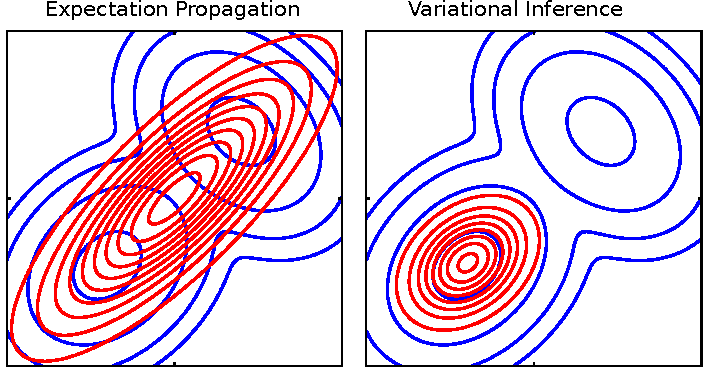
\includegraphics[width=.8\textwidth]{images/EPvsVI.pdf}
    \caption{An illustration~\cite{bishop:2006:PRML} of the behaviour of expectation propagation in comparison to variational inference. We see that EP tries to cover the whole probability mass whereas VI concentrates on the mode of one component.}
    \label{fig:EPvsVI}
\end{figure}

Despite all this, expectation propagation is often not suitable for the inference in Bayesian neural networks. 
This is because EP has to save every likelihood and prior factor in memory~\cite{minka2001expectation}.
Therefore, it does not scale well to large data sets and high model complexity and hence we will not go into detail.
In the next chapters, we present inference techniques which are slightly adapted versions of EP and address these problems.

\subsubsection{Probabilistic Backpropagation}
A variation of expectation propagation was proposed by Lobato et al.~\cite{hernandez2015probabilistic} and is named \textit{probabilistic backpropagation} (PBP).
In particular, it is a combination of EP and another related method that is called assumed density filtering~\cite{minka2001expectation}.

Similarly to the approaches described in Sec.~\ref{sec:variational_inference}, PBP makes the assumption of factorized distributions for the prior.
This leads to the posterior (already used in VI) which is given by
\begin{align}
    p(\boldsymbol{\omega} | \mathbf{X}, \mathbf{Y}) =
    p(\mathbf{Y} |\mathbf{X})^{-1}
    \underbrace{\prod_{n=1}^{N} \mathcal{N}\left( \mathbf{y}_n | f^{\boldsymbol{\omega}}\left( \mathbf{x}_n \right), \sigma^2 \right)}_{\text{Likelihood: } p(\mathbf{Y} | \mathbf{X}, \boldsymbol{\omega})}
    \underbrace{ \prod_{l}^{L} \prod_{i}^{K_l} \prod_{j}^{K_l-1}\mathcal{N}\left( w_{ij,l} | 0, 1\right)}_{\text{Prior: }p(\boldsymbol{\omega})} \label{eq:posterior_full}
\end{align}
where the variance $\sigma^2$ is a hyperparameter that must be specified by the user and represents the aleatoric uncertainty in the training data.
Besides that, PBP also assumes a factorized variational distribution which is given by
\begin{align}
    q_\theta\left(\boldsymbol{\omega}\right) = \prod_{l=1}^{L}\prod_{i=1}^{K_l}\prod_{j=1}^{K_{l-1}} \mathcal{N}\left( w_{ij,l} \mid \theta^\mathrm{mean}_{ij,l}, \theta^\mathrm{var}_{ij,l}\right)\label{eq:variational_factorized_bpb}.
\end{align}
In order to update the parameters $\theta$, we define the set 
\begin{align}
    \mathcal{J} = &\left\{ \mathcal{N}\left( \mathbf{y}_n | f^{\boldsymbol{\omega}}\left( \mathbf{x}_n \right), \sigma^2 \right) \,\middle|\, \forall (x_n, y_n) \in (\mathbf{X}, \mathbf{Y})\right\} \cup
    \left\{ \mathcal{N}\left( w_{ij,l}|0, 1\right) \,\middle|\, \forall w_{ij,l} \in \boldsymbol{\omega} \right\}
\end{align}
which contains all factors from likelihood and prior from Eq.~\ref{eq:posterior_full}.
Subsequently, we iterate over all distributions in $\mathcal{J}$ and minimize the KL-divergence given by
\begin{align}
    \theta^* = \underset{\theta}{\mathrm{argmin}}\  \mathrm{KL}\left(Z^{-1}f\cdot q_\theta(\boldsymbol{\omega})\right \| q_\theta(\boldsymbol{\omega})),
\end{align}
where $\theta^*$ represents the optimal solution, $f \in \mathcal{J}$ represents the current factor and $Z^{-1}$ depicts the normalization factor.
That is, we iteratively update the variational distribution by incorporating one factor from our posterior at a time.
Lobato et al.~\cite{hernandez2015probabilistic} estimated the normalization factor $Z$ since it does not have a closed form solution.
Additionally, they incorporated another prior distribution for the parameters of the factorized Gaussian prior $p(\boldsymbol{\omega})$ which we replaced with unit Gaussians for simplicity.

In contrast to PBP, EP removes the current factor from the posterior approximation which leads to improved accuracy. 
Nevertheless, it has the disadvantage that the approximate factors has to be kept in memory and thus we typically can not work with large data sets (GPU memory is often limited).

\subsubsection{Dropout with $\alpha$-divergences}
\label{sec:droput_alpha_divergence}
A generalization of the divergences considered so far is defined by Amari's $\alpha$-divergence~\cite{amari2012differential} given by
\begin{align}
    \mathrm{D}_{\alpha}(p \| q) = \frac{1}{\alpha(1 - \alpha)} \left(1 - \int p(\boldsymbol{\omega})^\alpha q_\theta(\boldsymbol{\omega})^{1 - \alpha} \mathrm{d}\boldsymbol{\omega}\right)\label{eq:alpha_divergence}
\end{align}
where $\alpha \in \mathbb{R}$ defines the dissimilarity behaviour.
That is, when considering $\alpha = 0$ we obtain the objective function $\mathrm{D}_0(p \| q) = \mathrm{KL}(q\|p)$, which is equivalent to the VI objective. 
In the case of $\alpha = 1$, we obtain $\mathrm{D}_1 = \mathrm{KL}(p\|q)$ which is equivalent to the EP objective.
Intuitively, high values of $\alpha$ tend to cover more probability mass whereas low values tend to concentrate on local modes as illustrated in Fig~\ref{fig:EPvsVI}.

Lobato et al.~\cite{hernandez2016black} proposed Blackbox-$\alpha$ that is based on the $\alpha$-divergence that is defined in \ref{eq:alpha_divergence}.
It uses a loss function that is easy to implement and can make use of libraries for automatic differentiation.
In particular, it is derived by assuming distributions from the exponential family, thus it takes the form 
\begin{align}
\mathcal{F}_\alpha (\theta) = - \frac{1}{\alpha} \sum_{n =1}^N \ln\mathbb{E}_{q_\theta(\mathbf{\omega})}\left[ \left( \frac{p(\mathbf{y}_n| f^{\boldsymbol{\omega}}(\mathbf{x}_n))p(\boldsymbol{\omega})^\frac{1}{N}}{q_\theta(\boldsymbol{\omega})^\frac{1}{N}}\right)^\alpha\right].\label{eq:alpha_divergence_objective}
\end{align}
This expectation is often intractable and can be approximated using Monte-Carlo integration which results in
\begin{align}
\mathcal{F}_\alpha (\theta) \approx - \frac{1}{\alpha} \sum_{n =1}^N \ln \frac{1}{K}\sum_{k=1}^K
\left[ \left( \frac{p(\mathbf{y}_n| f^{\boldsymbol{\omega}^{(k)}}(\mathbf{x}_n))p(\boldsymbol{\omega}^{(k)})^\frac{1}{N}}{q_\theta(\boldsymbol{\omega}^{(k)})^\frac{1}{N}}\right)^\alpha\right],\label{eq:alpha_divergence_objective_MC}
\end{align}
where $\omega^{(k)}$ are samples from the variational distribution $q_\theta(\boldsymbol{\omega})$.
As stated before, optimizing Eq.~\ref{eq:alpha_divergence_objective_MC} for different values of $\alpha$ leads to different behaviours of the variational distribution.

Extending on that, Li et al.~\cite{li2017dropout} combined Blackbox-$\alpha$ with dropout inference (Sec.~\ref{sec:dropout_inference}) to tackle the problem of underestimating uncertainty.
For that, they introduce cavity distributions in order to transform Eq.~\ref{eq:alpha_divergence_objective} to an equivalent objective that can be used with dropout given by
\begin{align}
    \mathcal{F}_{\alpha\text{-dropout}}(\theta) = -\frac{1}{\alpha} \sum_{n=1}^N \ln \sum_{k=1}^{K}\exp\left[-\alpha \cdot l\left(\mathbf{y}_n, f^{\boldsymbol{\omega}^{(k)}} (\mathbf{x}_n)\right) \right] + \mathrm{L}_2(\theta), \label{eq:dropout_alpha_divergence}
\end{align}
where $l$ defines the loss function (e.\,g., mean squared error), $\boldsymbol{\omega}^{(k)}$ are samples from the dropout variational distribution and $\mathrm{L}_2(\theta)$ defines the $L2$-regularization of the parameters from the network.

Note, in order to implement both loss functions in a numeric stable way, we need to make use of the so called \textit{log-sum-exp} trick. %which is shown in the appendix.
This is due to the factorized assumption for prior and variational distribution which will cause numerical issues.
Accordingly, we have to transform  Eq.~\ref{eq:alpha_divergence_objective_MC} by taking the exponential of the logarithm of the argument in the inner sum.
Equation~\ref{eq:dropout_alpha_divergence} does not need further transformation since it is already in a suitable form.
More details can be found in the appendix and in our implementation.

With the new objective given by Eq.~\ref{eq:dropout_alpha_divergence}, we can specify the behaviour of our variational distribution $q_\theta(\boldsymbol{\omega})$. 
In particular, we are now able to define a balance between uncertainty quality and predictive capability.
Lobato and Li both identified that using $\alpha=0.5$, which is equivalent to the Hellinger distance~\cite{li2017dropout}, yields good results in most applications.

% Variational inference and expectation propagation reformulate the inference task into an optimization problem.
% They belong to the deterministic methods for estimating the posterior.
% In particular, they assumed a variational distribution that has a simple form and therefore can not yield exact results.

\subsection{Markov Chain Monte-Carlo}
\label{sec:mcmc}
In contrast to deterministic methods, Markov chain Monte-Carlo (MCMC) methods describe stochastic approaches that yield exact results.
Such methods allow sampling from extremely complicated distribution such as the posterior from Eq.~\ref{eq:posterior} and scale well with a high dimensional sample space.
However, MCMC methods are really slow and require a lot of iterations for accurate results.
Besides that, it is often hard to determine the convergence of such methods.

In their usual form, MCMC algorithms start with a \textit{proposal distribution} $g(\boldsymbol{\omega} | \boldsymbol{\omega}^{(\tau)})$ that is dependent on another sample $\boldsymbol{\omega}^{(\tau)}$.
It is a simpler distribution from which we can easily draw samples.
Subsequently, we iteratively sample $\boldsymbol{\omega}^*$ from distribution $g(\boldsymbol{\omega} | \boldsymbol{\omega}^{(\tau)})$.
The sample is accepted if it fulfills a certain criterion which is usually defined by the algorithm.
If it is accepted, then we set $\boldsymbol{\omega}^{(\tau + 1)} = \boldsymbol{\omega}^*$ and repeat the procedure with the new proposal $g(\boldsymbol{\omega} | \boldsymbol{\omega}^{(\tau + 1)})$.
We discard it if the criterion is not fulfilled.
In this way, the samples $\boldsymbol{\omega}^{(1)}, \boldsymbol{\omega}^{(1)}, \ldots, \boldsymbol{\omega}^{(n)}$ that are drawn from the proposal distribution construct a Markov-Chain.
When doing this long for a long time, the stationary distribution of the Markov chain converges to the true distribution $p(\boldsymbol{\omega} | \mathbf{X}, \mathbf{Y})$.

One of the first approaches for MCMC in Bayesian NNs was proposed by Neal~\cite{Neal:1995:BLN:922680}. 
He uses a hybrid Monte-Carlo method which is an adaption of the Metropolis algorithm~\cite{metropolis1953equation} because ordinary MCMC methods that are commonly used in applications are very slow and suffer from random walk behaviour~\cite{bishop:2006:PRML}.
Furthermore, by using Gibbs sampling~\cite{Geman:1984:SRG:2286442.2286617} he also updates the hyperparameters.
The states $\boldsymbol{\omega}^{(1)}, \boldsymbol{\omega}^{(1)}, \ldots, \boldsymbol{\omega}^{(n)}$ are found by means of dynamic simulation.
However, it is batch method that can perform poorly on large data sets and needs problem specific parameter settings for training.

\section{Conclusion and Outlook}
\label{sec:conclusion_outlook}
In this work, we gave an foundation to Bayesian neural networks and linked their training with common inference techniques such as variational inference, expectation propagation and Markov chain Monte-Carlo.
Furthermore, we presented several important extensions in order to scale these techniques to the state-of-the-art field deep learning.

We conclude that the most promising framework for the training of Bayesian neural networks is probably dropout inference from Sec.~\ref{sec:dropout_inference}.
It has several advantages: 
\begin{itemize}
    \item It scales with complex models without the addition of further parameters.
    \item It scales with large amounts of data because the training is equivalent to the one of an ordinary neural network.
    \item It is easy to implement with state-of-the-art architectures like convolutional neural networks.
\end{itemize}
Therefore, it can be readily implemented for several tasks where uncertainty estimation plays an important role (i.\,e. active learning~\cite{settles2009active}).
Even though dropout inference does underestimate uncertainty, there are approaches like $\alpha$-divergences which tackle these problem.

Unfortunately, the other methods introduced above double the model complexity and the generalization to other architectures (convolutional neural networks) is not straight forward. 
For example, Markov chain Monte-Carlo methods often fail in combination with large data sets and need a lot of time for training.
Bayes-by-Backprop or Probabilistic Backpropagation do not scale with network complexity and therefore are hard to use in modern days of big data.

For future work, we aim to use dropout inference architectures for image recognition in an active learning setting.
With these technique, we should be able to obtain a good uncertainty estimation which takes an important role.
In particular, the $\alpha$-divergence seems to be promising since we can define a balance between uncertainty and predictive capability.

\bibliographystyle{splncs04}
\bibliography{aBib}

\end{document}